
%%%%%%%%%%%%%%%%%%%%%%%%
\subsection{Population-level Correlations between Parameters}
%%%%%%%%%%%%%%%%%%%%%%%%
\label{sec:Population-level correlations between parameters}

While much can be learned by studying the distributions of individual \ac{BBH} parameters, we can glean additional information on the population by considering how parameters are correlated with one another across systems.
In this subsection, we provide an overview of how parameters in the \ac{BBH} population appear to be broadly structured in various two-dimensional slices of parameter space, briefly discussing the astrophysical implications of our findings.

\subsubsection{Mass Ratio and Spin Correlations}
\label{subsubsec:mass_ratio_spin_correlations}
We begin by following up on the purported anti-correlation between \ac{BBH} mass ratio $q$ and effective inspiral spin $\chieff$.
\textbf{Although we find less support for the specific case of anti-correlation between $\bm{q}$ and $\bm{\chieff}$ relative to \gwtcthree, we find compelling evidence for some correlated structure in $\bm{(q,\chieff)}$.}
Namely, larger positive values of $\chieff$ appear to be favored as $q$ decreases, but it is unclear if this is accompanied by a preference for larger negative values of $\chieff$ as well.
The $(q,\chieff)$~\linearcorrelation~model imposes a linear functional dependence between \ac{BBH} mass ratio, and the mean and (natural log) width of the $\chieff$ distribution (see Appendix~\ref{appendix:LinearCorrelationModels}).
Fitting this model to \gwtcthree data suggests that a linear correlation coefficient of $\delta \mu_{\mathrm{eff}|q} < 0$ (i.e., the case of a negative $q$-dependence on the mean of the $\chieff$ distribution) with 98\% credibility \citep{KAGRA:2021duu}.
Updating this analysis to include data obtained over \ac{O4a} softens the evidence for an anti-correlation between $q$ and the mean of the $\chieff$ distribution, with a value of $\delta \mu_{\mathrm{eff}|q} < 0$ now inferred at $\qchieffLinearCorrelationModel[param][mu_chieff_1][percentile exclude zero]\%$ credibility.
However, we now see notable evidence for a linear increase in the log width of the $\chieff$ distribution as mass ratios become more unequal -- with $\delta \ln \sigma_{\mathrm{eff}|q} < 0$ at $\qchieffLinearCorrelationModel[param][ln_sigma_chieff_1][percentile exclude zero]\%$ credibility.

We plot the mass-ratio dependent mean and width of the $\chieff$ distribution inferred using the \linearcorrelation~model in Figure~\ref{fig:q_chieff_mu_sigma}.
In the bottom panel of Figure~\ref{fig:q_chieff_mu_sigma}, we include the two-dimensional posterior distribution of $\delta \mu_{\mathrm{eff}|q}$ and $\delta \ln \sigma_{\mathrm{eff}|q}$.
Inspecting this plot, we see an anti-correlation in the posterior of the two hyperparameters, where larger negative values of $\delta \mu_{\mathrm{eff}|q}$ imply values of $\delta \ln \sigma_{\mathrm{eff}|q}$ closer to zero, and larger negative values of $\delta \ln \sigma_{\mathrm{eff}|q}$ imply values of $\delta \mu_{\mathrm{eff}|q}$ closer to zero.
The case in which both parameters are zero (no correlation between $q$ and $\chieff$ of any kind) appears to be ruled out at $\approx 99\%$ credibility.
In practice, this implies that the \linearcorrelation~model finds support for larger positive values of $\chieff$ at more unequal mass ratios, but cannot yet conclude whether these are accompanied by larger negative values of $\chieff$ as well.

Next, we probe for more intricate correlations between $q$ and $\chieff$ using the \splinecorrelation~model.
Similar to the \linearcorrelation~model, the \splinecorrelation~model allows for the mean and width of the $\chieff$ distribution to evolve with mass ratio.
However, these mass ratio dependences, rather than being linear, are modeled flexibly with cubic splines \citep[see Appendix~\ref{appendix:LinearCorrelationModels} and][]{Heinzel:2023hlb}.
We plot the $q$-dependent means and widths inferred from the \splinecorrelation~model alongside those from the \linearcorrelation~model in Figure~\ref{fig:q_chieff_mu_sigma}.
Despite fluctuations emerging in the \splinecorrelation~model, the two models are, within \confidenceLevel~credible bounds, consistent.
The preference for broadening in the $\chieff$ distribution as $q$ decreases found with the \linearcorrelation~model, does not clearly appear in the \splinecorrelation~model.
In the bottom panel of Figure~\ref{fig:q_chieff_mu_sigma}, we also plot the inferred gradient of the $\chieff$ distribution's mean and (natural log) width relative to mass ratio at $q = 0.6$ (roughly the value at which covariance appears most pronounced).
Here, we see a similar structure to that of the \linearcorrelation~model's $(\delta \mu_{\mathrm{eff}|q}, \delta \ln \sigma_{\mathrm{eff}|q})$ posterior, albeit with much more uncertainty.
As a final observation from the \splinecorrelation~model in Figure~\ref{fig:q_chieff_mu_sigma}, we see that the inferred $\chieff$ distribution at low mass ratios ($q \lesssim 0.2$) grows in uncertainty, roughly recovering the prior.
This implies that any correlation inferred by the \linearcorrelation~model is likely driven by observations with mass ratios $q \gtrsim 0.2$.
As such, the inferences from this model should be interpreted with caution as $q \rightarrow 0$, where the trend is effectively being extrapolated from the more populated $q \gtrsim 0.2$ region due to a lack of model flexibility.

\begin{figure}
  \centering
  \includegraphics[width=0.6\columnwidth]{figures/correlation_spline_q_chi_eff.pdf}
  \caption{
  The inferred peak (top) and width (middle) of the $\chieff$ distribution as a function of mass ratio for the $(q,\chieff)$~\linearcorrelation~model (blue) and \splinecorrelation~model (orange).
  The shaded regions in these panels give the \confidenceLevel~credible intervals.
  The bottom panel gives the posterior distribution for the gradient of the $\chieff$ distribution's peak ($\delta \mu_{\mathrm{eff}|q}$) and natural log width ($\delta \ln \sigma_{\mathrm{eff}|q}$) dependent on mass ratio.
  From dark to light, the shaded regions represent the 50\%, 90\% and 99\% credible intervals.
  Again, blue gives the result of the \linearcorrelation~model, while orange shows the result of the \splinecorrelation~model sliced through $q=0.6$ (the approximate point at which the gradients are largest).
  It appears that mass ratio and $\chieff$ exhibit some kind of correlation, but the exact nature is unclear.
  }
  \label{fig:q_chieff_mu_sigma}
\end{figure}

We now move to the \copulacorrelation~model, which allows for a correlation between $q$ and $\chieff$ with a variable strength $\kappa_{q, \mathrm{eff}}$ (see Appendix~\ref{appendix:copulaCorrelationModels}).
This framework has the added advantage that the level of correlation is decoupled from the shape of the marginal distribution \citep[e.g.,][]{Adamcewicz:2022hce}, with less flexibility for covariant structure relative to other correlated population models.
Fitting the \copulacorrelation~model to \gwtcfour suggests that $q$ and $\chieff$ are anti-correlated ($\kappa_{q, \mathrm{eff}} < 0$) with $\qchieffCopulaCorrelationModel[param][kappa][correlated percentile]\%$ credibility.
Specifically, we infer $\kappa_{q, \mathrm{eff}} = \CIPlusMinus{\qchieffCopulaCorrelationModel[param][kappa]}$.
\cite{Adamcewicz:2023mov} analyzed \gwtcthree data with a copula model to find that $(q, \chieff)$ are anti-correlated with $>99\%$ credibility, suggesting greater evidence for an anti-correlation than is measured here.
However, these results are not directly comparable to those presented in this work, due to different modeling assumptions and different convergence criteria in the population likelihood.
Qualitatively, we see that the \copulacorrelation~model and \linearcorrelation~model exhibit a subtle anti-correlation in $(q, \chieff)$, as seen in the respective two-dimensional \acp{PPD} in Figure~\ref{fig:q_chieff_ppd}.

\begin{figure}
  \centering
  \includegraphics[width=0.6\columnwidth]{figures/q_chi_eff_ppd.pdf}
  \caption{
  Mass ratio and $\chieff$ \acp{PPD} for the \copulacorrelation~model (blue) and \linearcorrelation~model (orange).
  The contours, from dark to light, mark 50\%, 90\%, and 99\% of the volume.
  We see a subtle preference for an anti-correlation, although this feature is far less prevalent than it appeared in \gwtcthree.
  We also see evidence for a broadening in the distribution as mass ratios become more unequal in the \linearcorrelation~model.
  The \copulacorrelation~model is not flexible in a way that it can capture a broadening.
  }
  \label{fig:q_chieff_ppd}
\end{figure}

There are a number of potential astrophysical implications if the anti-correlation in $(q,\chieff)$ is real.
If isolated binaries make up a substantial fraction of the population and undergo tidal spin up, stable mass transfer and the resulting mass ratio reversal of systems \citep{Broekgaarden:2022nst, Zevin:2022wrw, Olejak:2024qxr} may produce an such an anti-correlation in the population.
This feature could also be explained by binaries undergoing a common-envelope phase provided common envelope efficiencies are sufficiently high \citep{Bavera:2020uch}.

Covariance in $(q,\chieff)$ could also be a result of hierarchical mergers contributing to a considerable fraction of the \ac{BBH} merger rate \citep{Antonini:2024het, Antonini:2025zzw}.
Hierarchical mergers should exhibit mass ratios that are more unequal and spin magnitudes that are larger than isolated, or first-generation dynamical mergers.
If hierarchical mergers occur in typical dynamical environments, the spins of the \acp{BH} will be isotropically distributed, thus producing a broadening in the $\chieff$ distribution as mass ratios become unequal.
Meanwhile, \acp{BH} in \ac{AGN} may have spins preferentially aligned with one another, meaning hierarchical mergers in these environments can produce a correlation between mass ratios and spins that is asymmetrical about $\chieff = 0$ \citep{McKernan:2021nwk, Santini:2023ukl}.
Stronger evidence for unequal mass binaries preferring positive values of $\chieff$ could then indicate that binaries merging in \ac{AGN} are predominantly coaligned with the rotation of the \ac{AGN} disk \citep{Santini:2023ukl}.

\subsubsection{Mass and Spin Correlations}
\label{subsubsec:mass_spin_correlations}
\textbf{We find model-dependent evidence for correlations between $\bm{m_1}$ and $\bm{\chieff}$.}
Motivated by the feature in the mass distribution around the ${\sim} 30{-}40 \,\Msun$ range, we use a \ac{BGP}~analysis allowing for correlations in $m_1$ and $\chieff$ (see Appendix~\ref{appendix:BGPModel}) to see if this feature in the distribution of masses is accompanied by a deviation in the \ac{BBH} spin distribution.
Using \gwtcfour, these studies find weak evidence that \ac{BBH} systems with at least one mass in the ${\sim} 30{-}40 \,\Msun$ peak tend to have spins that are symmetrically distributed about $\chieff = 0$, while binaries outside of this mass range have spins that are skewed toward positive (aligned) values of $\chieff$.
Quantitatively, this \ac{BGP}~analysis infers that for every merger in the ${\sim} 30{-}40 \,\Msun$ peak with a negative value of $\chieff$, there are $\CIPlusMinus{\MassSpinCorrelatedBGPModel[param][positive-to-negative chi_eff ratio for m in 30-40]}$ with a positive value of $\chieff$.
Meanwhile, for every event outside of this mass range with a negative value of $\chieff$, there are $\CIPlusMinus{\MassSpinCorrelatedBGPModel[param][positive-to-negative chi_eff ratio for m outside 30-40]}$ with a positive value of $\chieff$.
We illustrate this result in the top panel of Figure~\ref{fig:mass_spin_correlated_bgp_combined}.
Furthermore, in the \ac{BGP}~analysis the inferred distribution of masses for \ac{BBH} systems with effective inspiral spins ($|\chieff| \lesssim 0.1$) exhibits a preference for a larger proportion of mergers with $m_1 \sim 30{-}40 \,\Msun$, compared to systems with $\chieff \gtrsim 0.1$.
These distributions, however, remain consistent within \confidenceLevel~credible intervals.
This is illustrated in the bottom two panels of Figure~\ref{fig:mass_spin_correlated_bgp_combined}.
These features were also recovered with same analyses applied to \gwtcthree data, albeit with less certainty \citep{Ray:2024hos}.
However, more recent \gwtcthree analyses find conflicting evidence, suggesting that the $\chieff$ distribution of $\approx 30 \,\Msun$ \acp{BH} is positively skewed \citep{Sadiq:2025vly, Roy:2025ktr}.

\begin{figure}
	\centering
	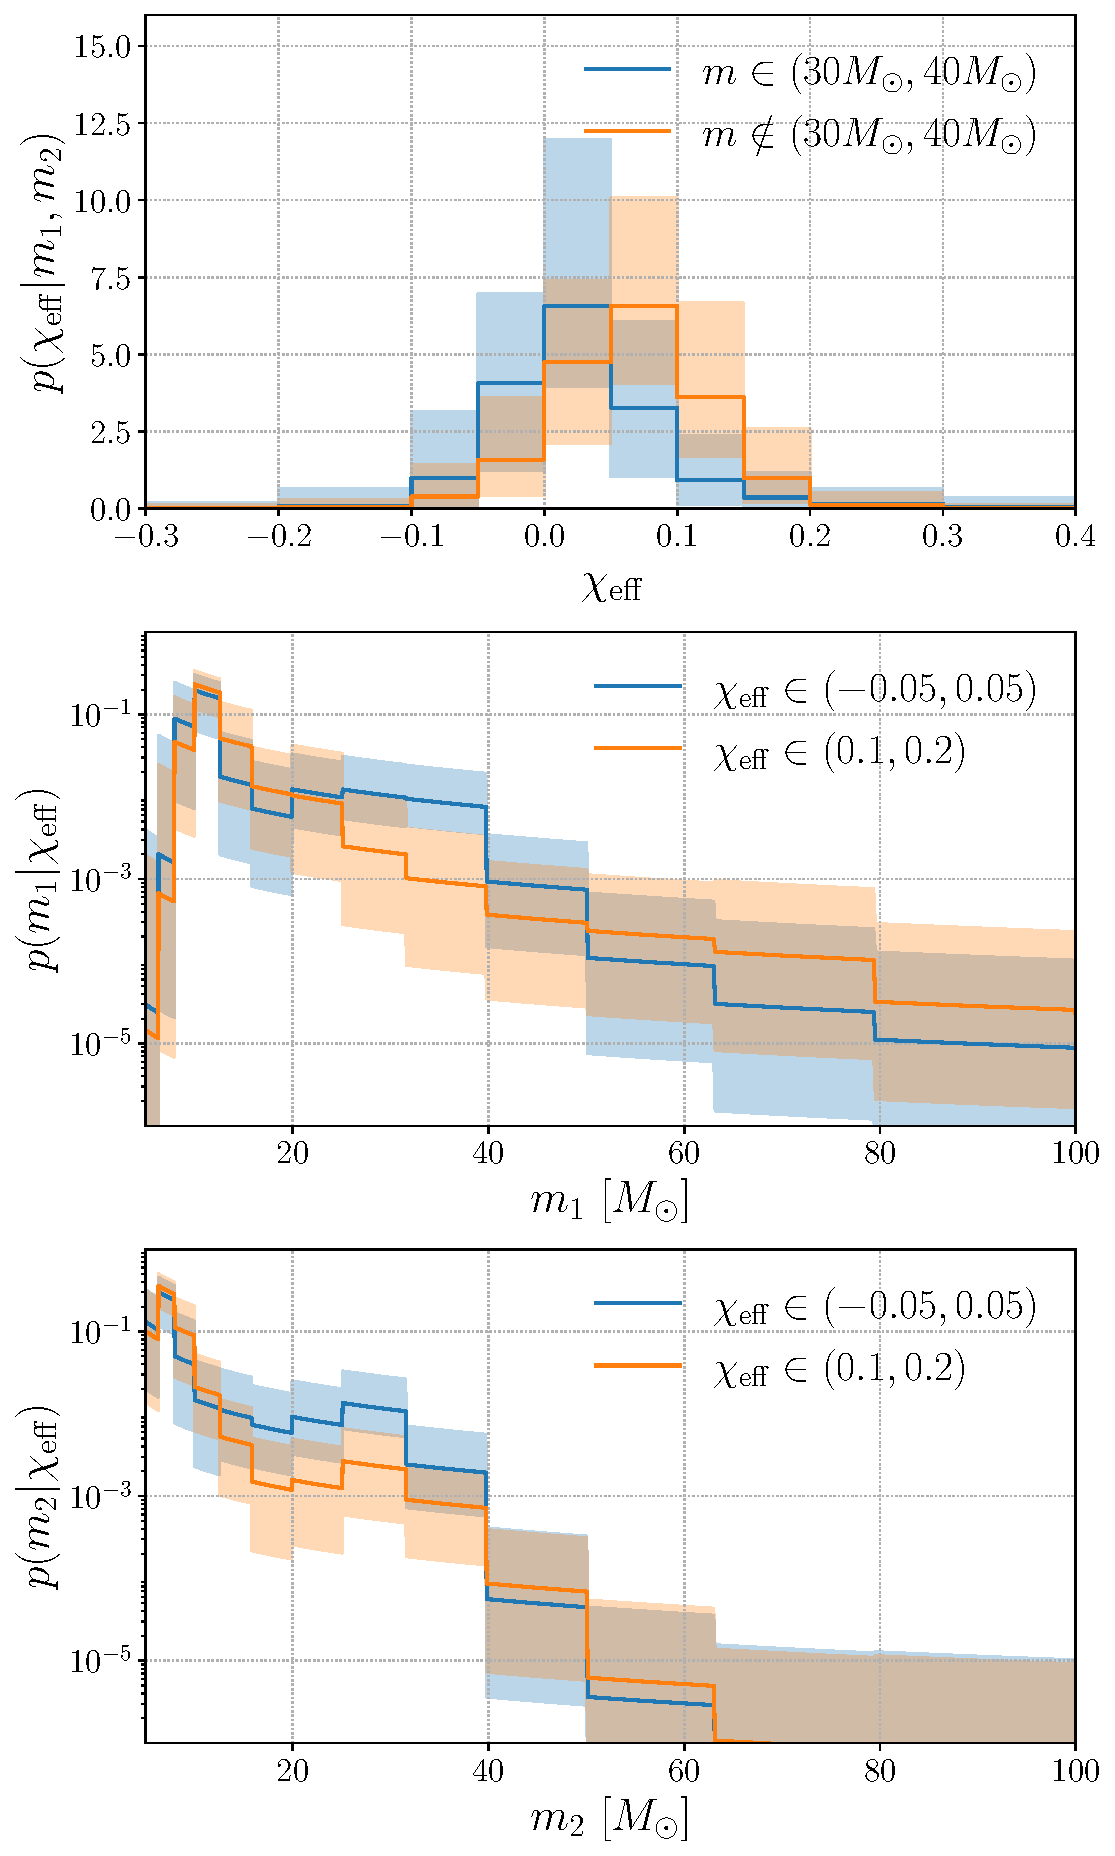
\includegraphics[width=0.5\columnwidth]{figures/mass_spin_correlated_bgp_combined.pdf}
	\caption{
  \textit{Top:} inferred distributions of effective inspiral spin $\chieff$ in the correlated mass--spin \ac{BGP}~analysis.
  The solid lines give the median, while the shaded regions indicate the \confidenceLevel~credible intervals.
  In blue, we have the $\chieff$ distribution of \ac{BBH} systems with at least one mass inside the $30{-}40 \,\Msun$ peak range.
	In orange, we have the $\chieff$ distribution of \ac{BBH} systems masses outside the $30{-}40 \,\Msun$ peak range.
  While the two distributions are consistent within \confidenceLevel~credible intervals, systems outside the peak range appear to favour a distribution of $\chieff$ skewed toward more positive values.
	Meanwhile, systems inside the peak range appear to favour a more symmetrical distribution about $\chieff = 0$.
  \textit{Middle:} inferred distributions of primary mass from the correlated mass--spin \ac{BGP}~analysis.
  \textit{Bottom:} inferred distributions of secondary mass from the correlated mass--spin \ac{BGP}~analysis.
	In both mass plots, blue shows the distribution for systems with small spins, $\chieff$ in the range $(-0.05,0.05)$, while orange shows the distribution for systems with larger spins, $\chieff$ in the range $(0.1,0.2)$.
	Note the preference for a higher proportion of mergers with masses $\approx 30{-}40 \,\Msun$ for low spin systems (blue).
	}
	\label{fig:mass_spin_correlated_bgp_combined}
\end{figure}

The \textsc{Isolated Peak}~model \citep[see also][]{Godfrey:2023oxb} fits the data to a model containing multiple mass subpopulations with independent spin distributions.
One subpopulation consists of a single peak in the mass distribution (which is inferred to center on ${\sim} 10 \,\Msun$), while other subpopulations are flexibly fit with the \BSpline~method.
Applying these analyses to \gwtcfour suggests that \acp{BH} within the ${\sim} 10 \,\Msun$ peak have a spin magnitude distribution consistent (within 90\% credibile intervals) with the rest of the \ac{BBH} population.
Meanwhile, although there is some overlap in the 90\% credibile regions of the cosine tilt distributions for both subpopulations, the distribution of tilts for \acp{BH} in the ${\sim} 10 \,\Msun$ peak favors alignment and is inconsistent with isotropy.
The distribution of cosine tilts for \acp{BH} outside this mass peak appears more symmetrical about $\cos \theta = 0$ and does not rule out isotropy.
Roughly speaking, this corresponds to a distribution of $\chieff$ that may be symmetrical about zero for the \ac{BBH} population outside of the ${\sim} 10 \,\Msun$ peak.
Inside this mass peak, however, the implied $\chieff$ distribution skews toward positive values.

We also model a correlation between primary mass and $\chieff$ using a copula model (see Appendix~\ref{appendix:copulaCorrelationModels}).
Fitting this \copulacorrelation~model with \gwtcfour data, we infer a correlation of $\kappa_{m_1, \mathrm{eff}} = \CIPlusMinus{\mchieffCopulaCorrelationModel[param][kappa]}$ between $m_1$ and $\chieff$.
Hence, the \copulacorrelation~analysis finds no evidence for a single, smooth, population-wide correlation between primary mass and $\chieff$.

Broadly, our analyses of the joint mass and spin distribution recover similar features to recent works that probe for features in \gwtcthree.
First, analyses of \gwtcthree do not find evidence for a smoothly correlated distribution in primary mass and $\chieff$ \citep{Safarzadeh:2020mlb, Biscoveanu:2022qac, Fishbach:2022lzq, Heinzel:2023hlb, Heinzel:2024hva, Antonini:2024het}, as is the case in this work.
Meanwhile, a number of analyses find evidence for separate subpopulations in mass and spin consistent with predictions of dynamical and field mergers.
More specifically, these works tend to find a subpopulation with lower masses and smaller, mostly aligned spins, and a second subpopulation of heavier binaries with larger, isotropically distributed spins, where the subpopulations transition around ${\sim} 40 \,\Msun$ \citep{Wang:2022gnx, Mould:2022ccw, Godfrey:2023oxb, Li:2023yyt, Antonini:2024het, Pierra:2024fbl, Guo:2024wwv, Li:2025rhu, Sadiq:2025vly}.
While the analyses presented in this work do not recover this exact feature (nor do they probe directly for it), the \textsc{Isolated Peak}~model's preference for aligned spins at ${\sim} 10 \,\Msun$ and isotropically distributed spins at higher masses may be related.

\subsubsection{Redshift and Spin Correlations}
\label{subsubsec:redshift_spin_correlations}
\textbf{We find evidence that the $\bm{\chieff}$ distribution broadens as redshift increases up to $\bm{z \sim 1}$}.
We again look for correlations between redshift and $\chieff$ by modeling the mean and width of the $\chieff$ distribution with a linear dependence on redshift (see Appendix~\ref{appendix:LinearCorrelationModels}).
\cite{Biscoveanu:2022qac} employed a \linearcorrelation~model for $(z,\chieff)$ to analyze \gwtcthree data, finding no evidence for redshift dependence in the mean of the $\chieff$ distribution, but suggesting that the $\chieff$ distribution broadens with increasing redshift ($\delta \ln \sigma_{\mathrm{eff}|z} > 0$ at 98.6\% credibility).
Updating this analysis to include \ac{O4a} data, we find more evidence for a broadening in the $\chieff$ distribution with redshift, with $\delta \ln \sigma_{\mathrm{eff}|z} > 0$ now inferred at $\zchieffLinearCorrelationModel[param][ln_sigma_chieff_1][percentile exclude zero]\%$ credibility.
The mean and width of the $\chieff$ distribution as functions of redshift are shown in Figure~\ref{fig:z_chieff_mu_sigma}.

The \splinecorrelation~model, which models the redshift dependence on the mean and width of the $\chieff$ distribution flexibly with cubic splines (see Appendix~\ref{appendix:SplineCorrelationModels}), is broadly consistent with the \linearcorrelation~model.
The exception is that the \splinecorrelation~model tends to recover the prior beyond a redshift of $z \gtrsim 1$.
This likely indicates that the \linearcorrelation~model is fitting a trend at low redshifts, then extending this trend to redshifts $z \gtrsim 1$ due to a lack of flexibility.
To further illustrate this point, the gray dashed line in Figure~\ref{fig:z_chieff_mu_sigma} indicates the redshift under which 90\% of the catalog's cumulative posterior support is contained.
Roughly speaking, this means our inferences above this redshift are informed by only ${\sim} 10\%$ of the data.
Therefore, while we find evidence that the $\chieff$ distribution broadens as binaries approach $z \sim 1$, we are unable to determine if this trend continues at higher redshifts.

We also model a correlation between redshift and $\chieff$ using a copula model, with variable correlation $\kappa_{z, \mathrm{eff}}$ (see Appendix~\ref{appendix:copulaCorrelationModels}).
In contrast to the above analyses, the \copulacorrelation~model finds evidence for a positive correlation in $(z,\chieff)$, inferring a value of $\kappa_{z, \mathrm{eff}} = \CIPlusMinus{\zchieffCopulaCorrelationModel[param][kappa]}$ (or $\kappa_{z, \mathrm{eff}} > 0$ with $\zchieffCopulaCorrelationModel[param][kappa][correlated percentile]\%$ credibility).
While the \copulacorrelation~model lacks the flexibility to fit a broadening directly, the long (albeit shallow) posterior tails reaching into both large-negative and large-positive values for $\kappa_{z, \mathrm{eff}}$ may relate to the broadening in the $\chieff$ distribution recovered by the \linearcorrelation~and~\splinecorrelation~models (see Appendix~\ref{appendix:supplementary_correlations}).
If the $z$-dependent broadening and constant mean of the $\chieff$ distribution from the \linearcorrelation~and~\splinecorrelation~models is to be believed, it is unclear why the posterior on $\kappa_{z, \mathrm{eff}}$ skews toward positive values, rather than being symmetric about zero.

\begin{figure}
  \centering
  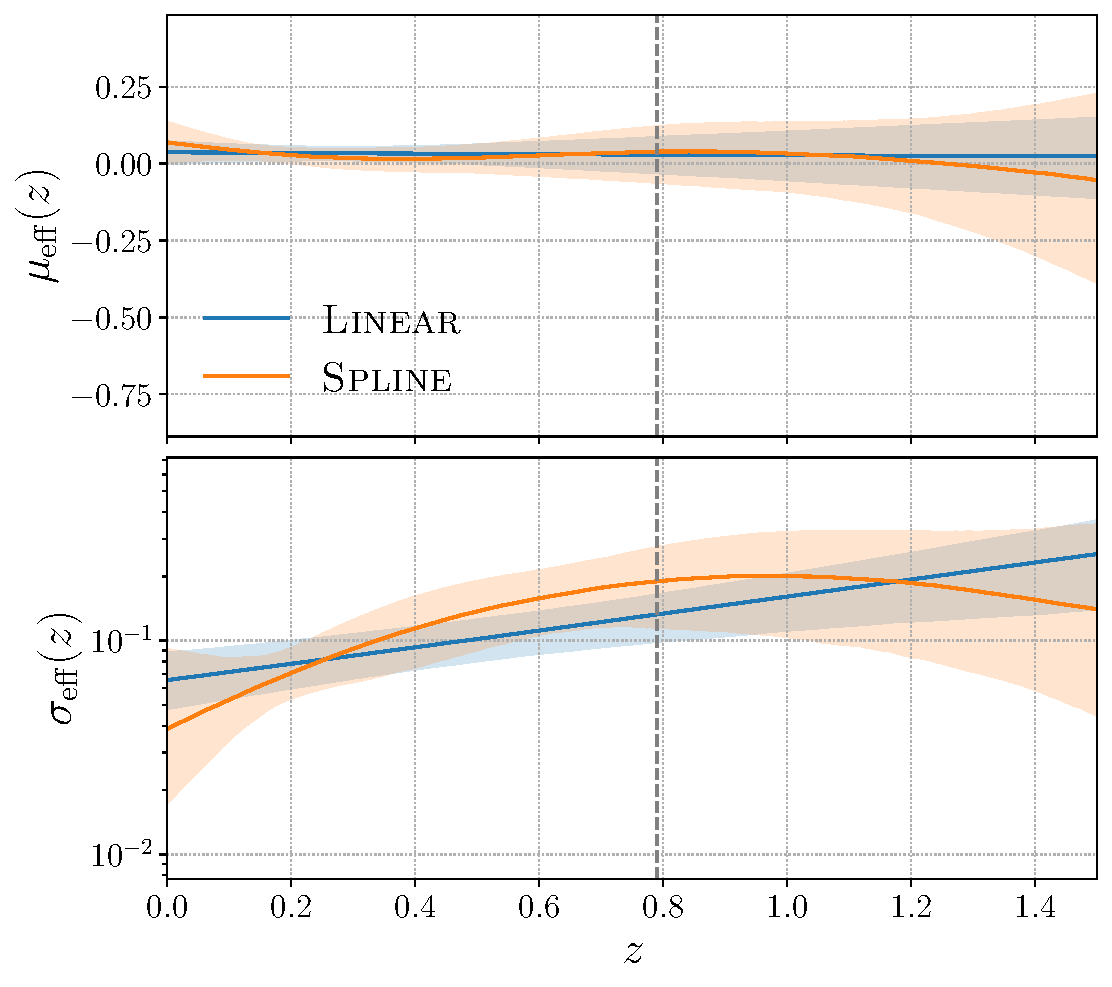
\includegraphics[width=0.6\columnwidth]{figures/correlation_spline_z_chi_eff.pdf}
  \caption{
  The inferred mean (top) and width (bottom) of the $\chieff$ distribution as a function of redshift for the \linearcorrelation~model (blue) and the \splinecorrelation~model (orange).
  The shaded regions give the \confidenceLevel~credible intervals.
  The gray dashed line indicates the redshift under which 90\% of the cumulative posterior probability lies across all events in \gwtcfour.
  Therefore, inferences above this redshift are dominated by the prior or population model.
  Note the logarithmic scale on the width (bottom panel).
  In either model, we find evidence that the width of the effective inspiral spin distribution increases with redshift up to $z \sim 1$.
  }
  \label{fig:z_chieff_mu_sigma}
\end{figure}

It is unclear what this broadening in the $\chieff$ distribution at greater redshifts might imply astrophysically.
Provided \ac{BH} progenitors experience significant spin up due to tidal torques, smaller orbital separations and periods will result in more efficient spin up of \ac{BBH} components \citep{Zaldarriaga:2017qkw, Mapelli:2018uds, Bavera:2020uch, Bavera:2022mef, Fuller:2022ysb}.
Of course, smaller orbital separations correspond to shorter delay-times to merger.
This means that these systems may contribute more to the merger rate in the earlier Universe (higher $z$), where systems with wider orbits have not had time to merge.
Furthermore, given that higher metallicity systems are expected to evolve to longer orbital periods due to experiencing more mass loss during core helium burning \citep{Qin:2018vaa, Fuller:2022ysb}, one might predict that larger spin magnitudes should be observed in regions of lower metallicity and thus also at higher redshifts.
However, the correlation in the \linearcorrelation~and~\splinecorrelation~models is between redshift and the width of the $\chieff$ distribution rather than the mean.
This includes an increasing number of systems with both large-positive and large-negative values of $\chieff$.
An increase in systems with large-negative $\chieff$ may be somewhat difficult to square with the above hypothesis, given that tidal spin up is only relevant in isolated systems, and that large supernovae kicks are required to misalign the \ac{BH} spins so significantly \citep{Kalogera:1999tq,  Wysocki:2017isg, Gerosa:2018wbw, Callister:2020vyz, Steinle:2020xej, Stevenson:2022hmi, Tauris:2022ggv, Baibhav:2024rkn}.
On the other hand, if the \copulacorrelation~results are to be taken at face-value, the preference for a positive correlation in $(z,\chieff)$ fits more neatly with the aforementioned hypothesis.

Another possibility, following discussion from Section~\ref{subsec:bbh_spins}, is that multiple separate subpopulations of \ac{BBH} mergers are being observed, where the more dominant (in terms of redshift-dependent merger rate) subpopulation changes at some nearby redshift.
Hierarchical mergers becoming more dominant at higher redshifts for example could potentially explain such a broadening in the effective spin distribution.
This interpretation would also imply some level of correlation between mass and redshift, which we do not find evidence for below in Section~\ref{subsubsec:redshift_mass_correlations}.

As a final caveat, using \gwtcthree data, \cite{Biscoveanu:2022qac} fit the \ac{BBH} population to a model in which the $\chieff$ distribution is linearly dependent on both primary mass and redshift.
In doing so, the authors find degeneracies between the $(m_1,\chieff)$ and $(z,\chieff)$ correlations.
While we do not explore correlations beyond two dimensions in this work, we acknowledge that the assumption of independence between other pairs of parameters may have notable effects on our inferences.

\subsubsection{Redshift and Mass Correlations}
\label{subsubsec:redshift_mass_correlations}
Finally, we consider potential correlations between BBH mass and redshift.
\textbf{We do not find evidence for evolution in the mass distribution with redshift.}
We emphasize that these inferences are constrained to the nearby Universe, with relatively little data beyond $z \sim 1$ (19 out of 153 \ac{BBH} events having posteriors consistent with $z>1$ to \confidenceLevel~credibility).
We model correlations between primary mass and redshift using a copula with correlation $\kappa_{m_1, z}$ (see Appendix~\ref{appendix:copulaCorrelationModels}).
Using this \copulacorrelation~model, we infer a correlation of $\kappa_{m_1, z} = \CIPlusMinus{\mzCopulaCorrelationModel[param][kappa]}$.
We also search for correlations between mass and redshift using a \ac{BGP}~analysis that allows for covariance in $m_1$ and $z$ (see Appendix~\ref{appendix:BGPModel}).
Similarly, this analysis finds that the mass distribution does not show a distinguishable evolution with redshift (see Appendix~\ref{appendix:supplementary_correlations}).
This conclusion is mostly in line with studies using \gwtcthree, which are also unable to infer any correlation between mass and redshift with confidence \citep{Fishbach:2021yvy, Sadiq:2021fin, vanSon:2021zpk, Karathanasis:2022rtr, Ray:2023upk, Heinzel:2023hlb, Heinzel:2024hva, Lalleman:2025xcs, Sadiq:2025aog}.
This is with the exception of \cite{Rinaldi:2023bbd} finding a positive correlation between \ac{BBH} primary mass and redshift, although a novel method is used to account for selection effects.

